\begin{figure}

\begin{minipage}{\linewidth}
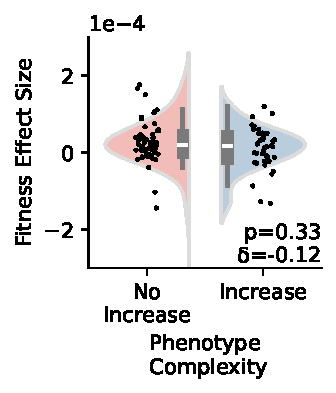
\includegraphics[width=0.39\linewidth]{%
binder-2025-09-05-genome-expansion-fitness/binder/teeplots/2025-09-05-genome-expansion-fitness/biotic_background=Contemporary+hue=phenotype-complexity+palette=pastel1+subject=Specimen+test=mw+viz=violinplot+what=phenotype+x=phenotype-complexity+y=fitness-differential-focal+ext=.pdf}
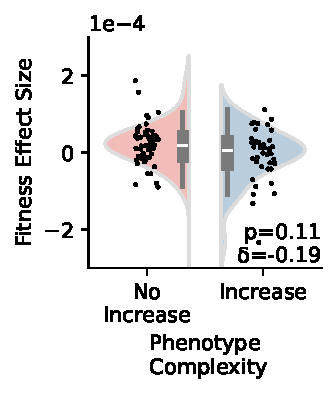
\includegraphics[width=0.305\linewidth, trim={1.3cm 0 0 0.6cm}, clip]{%
binder-2025-09-05-genome-expansion-fitness/binder/teeplots/2025-09-05-genome-expansion-fitness/biotic_background=Prefatory+hue=phenotype-complexity+palette=pastel1+subject=Specimen+test=mw+viz=violinplot+what=phenotype+x=phenotype-complexity+y=fitness-differential-focal+ext=.pdf}%
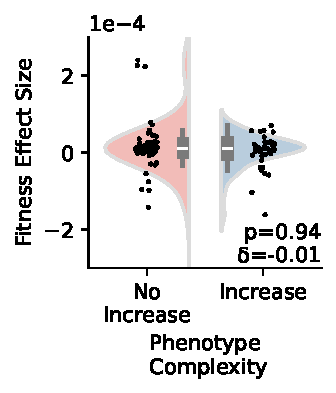
\includegraphics[width=0.305\linewidth, trim={1.3cm 0 0 0.6cm}, clip]{%
binder-2025-09-05-genome-expansion-fitness/binder/teeplots/2025-09-05-genome-expansion-fitness/biotic_background=Without+hue=phenotype-complexity+palette=pastel1+subject=Specimen+test=mw+viz=violinplot+what=phenotype+x=phenotype-complexity+y=fitness-differential-focal+ext=.pdf}

\vspace{-1ex}

\begin{subfigure}{0.135\linewidth}
~
\end{subfigure}%
\begin{subfigure}{0.305\linewidth}
    \centering
    \caption{\footnotesize specimen\\contemporary\\background}
    \label{fig:fitness-pcomplexity:specimen-contemporary}
\end{subfigure}%
\begin{subfigure}{0.305\linewidth}
    \centering
    \caption{\footnotesize specimen\\prefatory\\background}
    \label{fig:fitness-pcomplexity:specimen-prefatory}
\end{subfigure}%
\begin{subfigure}{0.255\linewidth}
    \centering
    \caption{\footnotesize specimen\\without\\background}
    \label{fig:fitness-pcomplexity:specimen-without}
\end{subfigure}
\end{minipage}

\begin{minipage}{\linewidth}
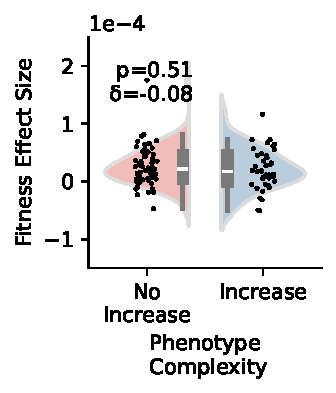
\includegraphics[width=0.39\linewidth]{%
binder-2025-09-05-genome-expansion-fitness/binder/teeplots/2025-09-05-genome-expansion-fitness/biotic_background=Contemporary+hue=phenotype-complexity+palette=pastel1+subject=Population+test=mw+viz=violinplot+what=phenotype+x=phenotype-complexity+y=fitness-differential-focal+ext=.pdf}
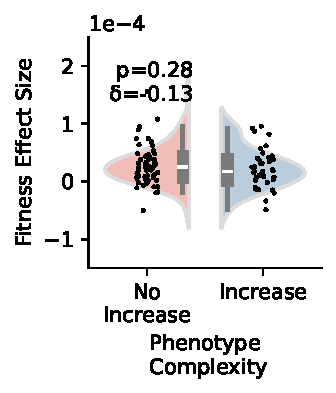
\includegraphics[width=0.305\linewidth, trim={1.3cm 0 0 0.6cm}, clip]{%
binder-2025-09-05-genome-expansion-fitness/binder/teeplots/2025-09-05-genome-expansion-fitness/biotic_background=Prefatory+hue=phenotype-complexity+palette=pastel1+subject=Population+test=mw+viz=violinplot+what=phenotype+x=phenotype-complexity+y=fitness-differential-focal+ext=.pdf}%
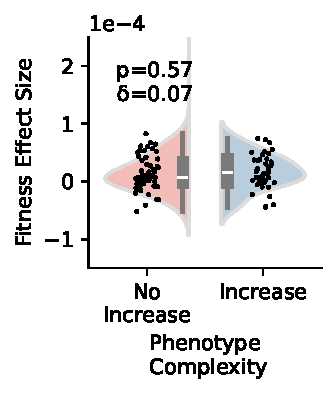
\includegraphics[width=0.305\linewidth, trim={1.3cm 0 0 0.6cm}, clip]{%
binder-2025-09-05-genome-expansion-fitness/binder/teeplots/2025-09-05-genome-expansion-fitness/biotic_background=Without+hue=phenotype-complexity+palette=pastel1+subject=Population+test=mw+viz=violinplot+what=phenotype+x=phenotype-complexity+y=fitness-differential-focal+ext=.pdf}

\vspace{-1ex}

\begin{subfigure}{0.135\linewidth}
~
\end{subfigure}%
\begin{subfigure}{0.305\linewidth}
    \centering
    \caption{\footnotesize population\\contemporary\\background}
    \label{fig:fitness-pcomplexity:population-contemporary}
\end{subfigure}%
\begin{subfigure}{0.305\linewidth}
    \centering
    \caption{\footnotesize population\\prefatory\\background}
    \label{fig:fitness-pcomplexity:population-prefatory}
\end{subfigure}%
\begin{subfigure}{0.255\linewidth}
    \centering
    \caption{\footnotesize population\\without\\background}
    \label{fig:fitness-pcomplexity:population-without}
\end{subfigure}
\end{minipage}


\caption{
    \textbf{Co-occurence of adaptation and changes in phenotypic complexity.}
    \footnotesize
    Violin plots compare adaptation assay outcome distributions between focal specimens with phenotype complexity (critical cardinal interface count) increase relative to ancestor and those without.
    Assays compete either focal specimen or focal population at stint $n+1$ against focal population at stint $n$;
    panels report outcomes under three assay designs, differing in biotic context.
    Contemporary competitons included background strain population from stint $n+1$, prefatory competitions included background strain population from stint $n$.
    Competitions without biotic background had no background strain participation.
    Reported statistics are Cliff's delta, a non-parametric effect size metric ranging from 0.0 to 1.0, and two-tailed Mann-Whitney U test.
}
\label{fig:fitness-pcomplexity}

\end{figure}
